% 第6章第5节：图傅里叶变换（谱坐标与重构、环图上的傅里叶基）。

\section{图傅里叶变换}
\label{sec:graph-fourier-transform}
\label{sec:signal-analysis-graph-state-kernels}

上一节的特征向量按变化尺度排成一组标准正交基。本节把顶点函数展开在这组基上：先建立投影系数、重构公式和两种能量的分解，再在规则的环图上说明熟悉的复指数为什么恰好是特征向量。所用的只是有限维正交分解与复数运算，离散傅里叶变换和快速算法留给后续信号部分。

\subsection{谱坐标与重构}
\label{sec:graph-spec-spectral-coordinates}

给定$\bm L$的一组标准正交特征向量$\bm u_1,\ldots,\bm u_n$，按特征值从小到大排成正交矩阵$\bm U$。任意顶点函数都可以在这组基下写出坐标，坐标就是它与各基向量的内积（第~\ref{sec:ls-orthonormal-bases}节）。

\begin{definition}[图傅里叶变换]
\label{def:graph-spec-graph-fourier-transform}
设$\bm L=\bm U\bm\Lambda\bm U^{\top}$为式~\eqref{eq:graph-spec-laplacian-eigendecomposition}的谱分解。顶点函数$\bm f$的\term{图傅里叶变换}（graph Fourier transform）及其逆变换为
\begin{equation}
 \widehat{\bm f}=\bm U^{\top}\bm f,\qquad \bm f=\bm U\widehat{\bm f}=\sum_{k=1}^n\widehat f_k\bm u_k ,
 \label{eq:graph-spec-graph-fourier-transform}
\end{equation}
其中$\widehat f_k=\bm u_k^{\top}\bm f$称为$\bm f$的第$k$个\term{谱坐标}（spectral coordinate）。
\end{definition}

正变换逐个读出$\bm f$在各模态方向上的分量，逆变换再把这些分量乘回对应的基向量相加。因为$\bm U^{\top}\bm U=\bm U\bm U^{\top}=\bm I$，两步互为逆运算，完整换坐标不丢失任何信息。

\begin{figure}[!htb]
  \centering
  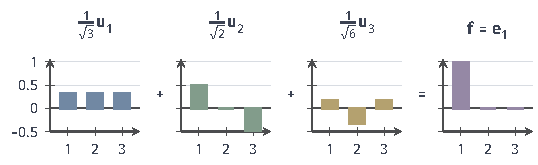
\includegraphics[width=91mm]{figures/01-basic-mathematics/04-graphs/tikz/c6-spectral-projection/figure.pdf}
  \caption{三点路径上单位脉冲的谱展开。前三幅是各模态乘以对应谱坐标后的贡献$\widehat f_k\bm u_k$，分别为$(\tfrac13,\tfrac13,\tfrac13)$、$(\tfrac12,0,-\tfrac12)$与$(\tfrac16,-\tfrac13,\tfrac16)$；逐点相加恰好恢复第四幅的$\bm e_1=(1,0,0)^{\top}$。}
  \label{fig:graph-spec-spectral-projection}
\end{figure}

在单位权三点路径上用第~\ref{sec:graph-spec-eigenvectors-scales}小节的三个模态展开单位脉冲$\bm f=\bm e_1$。三个谱坐标是$\bm u_k$的第一个分量：
\[
 \widehat{\bm f}=\Bigl(\tfrac1{\sqrt3},\tfrac1{\sqrt2},\tfrac1{\sqrt6}\Bigr)^{\top}.
\]
重构时，三个贡献分别是$\tfrac1{\sqrt3}\bm u_1=\tfrac13(1,1,1)^{\top}$、$\tfrac1{\sqrt2}\bm u_2=\tfrac12(1,0,-1)^{\top}$、$\tfrac1{\sqrt6}\bm u_3=\tfrac16(1,-2,1)^{\top}$。第一个分量相加为$\tfrac13+\tfrac12+\tfrac16=1$，第二个为$\tfrac13+0-\tfrac13=0$，第三个为$\tfrac13-\tfrac12+\tfrac16=0$，恰好回到$\bm e_1$，见图~\ref{fig:graph-spec-spectral-projection}。一个集中在一点的函数，需要全部三个模态共同表示。

\paragraph{两种能量的分解}
谱坐标把两种不同的“大小”都拆成逐模态的和。由$\bm U$正交，$\lVert\bm f\rVert_2^2=\lVert\bm U^{\top}\bm f\rVert_2^2$；把$\bm f=\bm U\widehat{\bm f}$代入二次型，交叉项消失（式~\eqref{eq:matrix-analysis-quadratic-spectral-form}）。于是
\begin{equation}
 \lVert\bm f\rVert_2^2=\sum_{k=1}^n\widehat f_k^{\,2},\qquad
 \bm f^{\top}\bm L\bm f=\sum_{k=1}^n\lambda_k\widehat f_k^{\,2}.
 \label{eq:graph-spec-parseval}
\end{equation}
前者是总幅值的平方，各模态平等计入；后者是沿边变化能量，每个模态按自己的特征值加权。对上面的脉冲，$\tfrac13+\tfrac12+\tfrac16=1$，能量为$0\cdot\tfrac13+1\cdot\tfrac12+3\cdot\tfrac16=1$，与直接计算一致：只有边$\{1,2\}$上有差$1$。再取$\bm f=(3,1,2)^{\top}$，谱坐标为$(2\sqrt3,\tfrac1{\sqrt2},\tfrac{\sqrt6}2)^{\top}$，平方和$12+\tfrac12+\tfrac32=14=3^2+1^2+2^2$，能量$0+\tfrac12+3\cdot\tfrac32=5$，与第~\ref{sec:graph-spec-dirichlet-energy}小节的结果相同。这个函数的幅值主要在常量模态上，能量却主要来自高频模态$\bm u_3$。

只保留前$r$个模态，得到$\bm f_r=\sum_{k\leq r}\widehat f_k\bm u_k$。它是$\bm f$在$\operatorname{span}\{\bm u_1,\ldots,\bm u_r\}$上的正交投影（第~\ref{sec:ls-projection-matrices}节），误差平方为$\lVert\bm f-\bm f_r\rVert_2^2=\sum_{k>r}\widehat f_k^{\,2}$。例如$\bm f=(3,1,2)^{\top}$保留前两个模态得$(2,2,2)^{\top}+\tfrac12(1,0,-1)^{\top}=(\tfrac52,2,\tfrac32)^{\top}$，误差平方为$\tfrac32$。截断后丢掉的分量无法恢复，所以这是投影近似，不再是完整的可逆变换。

\paragraph{基的选择自由}
谱坐标依赖所选的基。每个特征向量都可以换成它的相反数，相应的谱坐标随之变号。特征值有重复时自由更大：对应特征空间中的任意一组标准正交基都可以使用，单个谱坐标随基的选取改变。不随基改变的是到每个特征空间的投影，以及同一特征值的谱坐标平方和。所以比较两次计算的谱坐标时，应比较特征子空间上的投影，或者记录所用的基，不能只比较“第$k$个数”。下文的四点环有一对重复特征值，就属于这种情形。

\paragraph{计算代价}
取得谱基本身有代价。对稠密的$n\times n$对称矩阵作完整特征分解，通常需要$O(n^3)$次运算，存储$\bm U$需要$O(n^2)$空间；有了$\bm U$之后，每次正变换或逆变换是一次稠密矩阵乘向量，需要$O(n^2)$次运算。核算时要把两部分分开，不能把预先给定的谱基当作没有成本。大图上常常只求少数几个特征向量，那时得到的是截断投影，不是完整的变换。

\subsection{环图上的傅里叶基}
\label{sec:graph-spec-cycle-fourier-basis}

一般图的特征向量需要数值计算，但规则的环图可以直接写出来。取$N\geq3$个顶点的单位权简单环，顶点按环上次序编号为$r=0,1,\ldots,N-1$，下标按模$N$理解，即顶点$r$与$r\pm1$相邻。每个顶点的度为$2$，拉普拉斯逐点作用为
\[
 (\bm L\bm f)[r]=2f[r]-f[r-1]-f[r+1].
\]
环上每个顶点看到的局部结构都一样，这提示尝试沿环匀速旋转的复指数。对$k=0,1,\ldots,N-1$，令
\begin{equation}
 u_k[r]=\frac1{\sqrt N}\,\mathrm e^{2\pi\mathrm ikr/N}.
 \label{eq:graph-spec-cycle-eigenvector}
\end{equation}
代入并提出公因子$u_k[r]$，再用Euler公式（定理~\ref{thm:ru-euler-formula}）得$\mathrm e^{\mathrm i\theta}+\mathrm e^{-\mathrm i\theta}=2\cos\theta$，于是
\[
 (\bm L\bm u_k)[r]=u_k[r]\bigl(2-\mathrm e^{-2\pi\mathrm ik/N}-\mathrm e^{2\pi\mathrm ik/N}\bigr)
 =\Bigl(2-2\cos\frac{2\pi k}N\Bigr)u_k[r].
\]
所以$\bm u_k$是特征向量，特征值为$\lambda_k=2-2\cos(2\pi k/N)$。环的循环下标保证了$r=0$与$r=N-1$处的计算与其他位置相同，因为$\mathrm e^{2\pi\mathrm ikN/N}=1$。

这些向量是复向量，正交性要用复内积$\langle\bm x,\bm y\rangle=\bm x^*\bm y$来检验，其中$^*$表示共轭转置（第~\ref{sec:ls-inner-product-definition}节）。对$0\leq k,l\leq N-1$，
\[
 \langle\bm u_k,\bm u_l\rangle=\frac1N\sum_{r=0}^{N-1}\mathrm e^{2\pi\mathrm i(l-k)r/N}.
\]
$l=k$时每项为$1$，和为$1$。$l\neq k$时令$\rho=\mathrm e^{2\pi\mathrm i(l-k)/N}$，由$0<|l-k|<N$知$\rho\neq1$，而$\rho^N=1$；有限几何和公式（式~\eqref{eq:prelim-finite-geometric-sum}）的推导只用到乘法与减法，对复数公比同样成立，于是和为$(1-\rho^N)/(1-\rho)=0$。所以$\bm u_0,\ldots,\bm u_{N-1}$是$\mathbb C^N$的标准正交基，排成的矩阵$\bm U$满足$\bm U^*\bm U=\bm I$，是酉矩阵（第~\ref{sec:ls-adjoints}节）。相应地，正变换必须使用共轭转置：
\[
 \widehat{\bm f}=\bm U^*\bm f,\qquad \bm f=\bm U\widehat{\bm f},\qquad \lVert\bm f\rVert_2^2=\sum_k|\widehat f_k|^2 .
\]
$\bm L$是实对称矩阵，也有实的特征向量，例如$\bm u_k$与$\bm u_{N-k}$的实部和虚部；用复指数只是因为它对所有$k$给出统一的公式。

\begin{figure}[!htb]
  \centering
  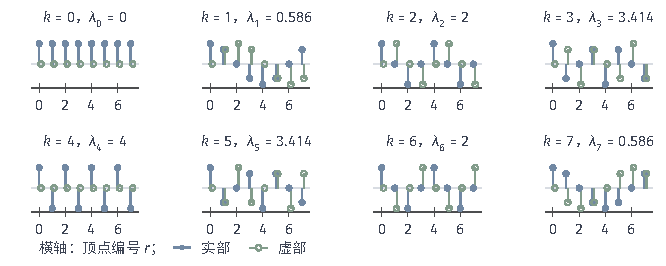
\includegraphics[width=112mm]{figures/01-basic-mathematics/04-graphs/tikz/c6-cycle-fourier-basis/figure.pdf}
  \caption{八点单位权环的复指数特征向量$u_k[r]=\mathrm e^{2\pi\mathrm ikr/8}/\sqrt8$。蓝色实心为实部，绿色空心为虚部，横轴为顶点编号$r$，标题给出特征值$\lambda_k=2-2\cos(2\pi k/8)$。$k$与$8-k$的实部相同、虚部相反，特征值相等；按$k$排列时特征值先增后减，$k=4$的振荡最快。}
  \label{fig:graph-spec-cycle-fourier-basis}
\end{figure}

图~\ref{fig:graph-spec-cycle-fourier-basis}画出$N=8$时的全部八个特征向量。编号$k$是复振荡沿环转动的圈数，不是特征值的次序：特征值随$k$先增后减，$k$与$N-k$给出相同的特征值。原因是$\bm u_{N-k}=\overline{\bm u_k}$，二者沿相反方向转动，相邻顶点间的差异一样大。

\paragraph{四点环上的单位脉冲}
取$N=4$，此时$u_k[r]=\tfrac12\mathrm i^{kr}$，特征值依次为$\lambda_0=0$、$\lambda_1=2$、$\lambda_2=4$、$\lambda_3=2$，其中$\lambda_1=\lambda_3$是一对重复特征值。对顶点$0$上的单位脉冲$\bm f=\bm e_0$，
\[
 \widehat f_k=\sum_r\overline{u_k[r]}f[r]=\overline{u_k[0]}=\tfrac12,\qquad k=0,1,2,3 ,
\]
四个谱坐标都是$\tfrac12$。重构时，$f[r]=\sum_k\tfrac12\cdot\tfrac12\mathrm i^{kr}=\tfrac14\sum_{k=0}^3\mathrm i^{kr}$：$r=0$时为$1$；$r=1,2,3$时公比$\mathrm i^r\neq1$且$(\mathrm i^r)^4=1$，几何和为零。于是恢复了$\bm e_0$。若把脉冲移到顶点$1$，谱坐标变为$\overline{u_k[1]}=\tfrac12\mathrm i^{-k}$，即$\tfrac12,-\tfrac{\mathrm i}2,-\tfrac12,\tfrac{\mathrm i}2$：模都不变，只是辐角随$k$转动。沿环平移只改变各谱坐标的相位，这正是复指数基在环上的方便之处。

这组复指数与信号处理中离散傅里叶变换使用的振荡是同一组，只差归一化常数$\sqrt N$。完整的离散傅里叶变换及其快速算法由后续信号部分展开。环的特殊之处在于存在把每个顶点移到下一个顶点的平移，复指数正是在平移下只改变相位的函数；一般图没有这样的平移，按顶点编号对数组做快速傅里叶变换，得不到该图拉普拉斯的谱坐标。
